\section{Model problem and notation}

We consider the constant-coefficient advection equation
\begin{equation}
 u_t+a u_x=0,
 \qquad a>0,
 \qquad 0\leq x\leq D,
 \qquad t>0,
\end{equation}
with initial condition
\begin{equation}
 u(x,0)=0
\end{equation}
and an incoming wave at the left boundary,
\begin{equation}
 u(0,t)=g(t).
\end{equation}
The two boundary functions are
\begin{align}
 g_{\sin}(t)&=\sin\!\left(\frac{2\pi t}{\tau}\right),\\
 g_{\mathrm{sq}}(t)&=\operatorname{sign}\!\left(
 \sin\!\left(\frac{2\pi t}{\tau}\right)\right).
\end{align}
The parameters used in the experiments are
\[
 \tau=2,
 \qquad D=10,
 \qquad a=2,
 \qquad 0\leq t\leq4.
\]

On the uniform grid we write
\begin{equation}
 x_j=jh,
 \qquad t_n=nk,
 \qquad u_j^n\approx u(x_j,t_n),
 \qquad \lambda=\frac{ak}{h}.
\end{equation}
The dimensionless number $\lambda$ is the CFL number. It measures how far the
physical wave travels during one time step relative to one spatial grid cell.

\section{Part 1(a): characteristics and the exact solution}

\subsection{Characteristic curves}

Let a curve in the $(x,t)$ plane be parameterized by
\[
 s\longmapsto (X(s),T(s)).
\]
The value of the solution along this curve is
\[
 U(s)=u(X(s),T(s)).
\]
By the chain rule,
\begin{equation}
 \frac{\dd U}{\dd s}
 =u_x(X(s),T(s))X'(s)+u_t(X(s),T(s))T'(s).
\end{equation}
We are free to use time itself as the curve parameter, so we set
\[
 T(s)=s,
 \qquad T'(s)=1.
\]
If we then choose
\[
 X'(s)=a,
\]
the derivative along the curve becomes
\begin{equation}
 \frac{\dd U}{\dd s}=u_t+a u_x=0.
\end{equation}
Thus $u$ is constant along every characteristic. Integration of $X'(s)=a$
gives
\begin{equation}
 X(s)-as=C,
\end{equation}
so the characteristics are straight lines $x-at=C$ with speed $a$.

To find the value at a particular point $(x,t)$, the characteristic through
that point is
\begin{equation}
 X(s)=x-a(t-s).
\end{equation}
We trace this line backward until it reaches data that are already known.

\subsection{Which data are reached first?}

At the initial line $s=0$, the characteristic is at
\[
 X(0)=x-at.
\]
There are two cases:
\begin{enumerate}
 \item If $x-at\geq0$, the characteristic reaches the initial line inside the
 domain. Since $u(X(0),0)=0$, the solution is zero.
 \item If $x-at<0$, the characteristic must cross the left boundary before it
 reaches $t=0$. Solving $X(s_b)=0$ gives
 \[
 s_b=t-\frac{x}{a}.
 \]
 The solution therefore equals the prescribed boundary value $g(s_b)$.
\end{enumerate}
Hence the exact finite-domain solution is
\begin{equation}
 \boxed{
 u(x,t)=
 \begin{cases}
 g\!\left(t-\dfrac{x}{a}\right),&0\leq x<at,\\[2mm]
 0,&at\leq x\leq D.
 \end{cases}}
 \label{eq:exact-solution}
\end{equation}

The sign of $a$ decides where information enters the domain. Here $a>0$, so
characteristics travel from left to right and the physical boundary condition
belongs at $x=0$. No physical condition is prescribed at $x=D$ because
characteristics leave the domain there.

At $t=4$, the leading characteristic has reached
\[
 x=at=8.
\]
For the sine boundary condition, equation~\eqref{eq:exact-solution} becomes
\begin{equation}
 u(x,4)=
 \begin{cases}
 -\sin(\pi x/2),&0\leq x<8,\\
 0,&8\leq x\leq10.
 \end{cases}
 \label{eq:exact-sine-t4}
\end{equation}
This gives the sequence $0,-1,0,1,0,-1,0,1,0$ at the integer positions
$x=0,1,\ldots,8$, which provides a direct check of the numerical plots.

\section{Finite-difference methods}

\subsection{Upwind method}

Because $a>0$, information at $x_j$ comes from the left. We therefore combine
a forward difference in time with a backward difference in space:
\begin{equation}
 \frac{u_j^{n+1}-u_j^n}{k}
 +a\frac{u_j^n-u_{j-1}^n}{h}=0.
\end{equation}
Solving for the new value gives
\begin{equation}
 \boxed{u_j^{n+1}
 =u_j^n-\lambda(u_j^n-u_{j-1}^n)
 =(1-\lambda)u_j^n+\lambda u_{j-1}^n.}
 \label{eq:upwind}
\end{equation}
For $0\leq\lambda\leq1$, this is a convex combination of two old values.
Consequently the method does not create new maxima or minima. It is robust at
discontinuities, but the averaging causes numerical smearing.

\subsection{Lax--Friedrichs method}

The centered approximation of $u_x$ is combined with the average of the two
neighboring values:
\begin{equation}
 \boxed{u_j^{n+1}
 =\frac{u_{j+1}^n+u_{j-1}^n}{2}
 -\frac{\lambda}{2}(u_{j+1}^n-u_{j-1}^n).}
 \label{eq:lax-friedrichs}
\end{equation}
The first term is an explicit spatial average. This stabilizes the centered
difference, but it also introduces substantial numerical diffusion.

\subsection{Lax--Wendroff method}

Taylor expansion about $(x_j,t_n)$ gives
\begin{equation}
 u(x_j,t_n+k)
 =u+k u_t+\frac{k^2}{2}u_{tt}+\bigO(k^3).
\end{equation}
From the PDE,
\[
 u_t=-a u_x,
 \qquad
 u_{tt}=-a(u_x)_t=-a(u_t)_x=a^2u_{xx}.
\]
Using centered differences for $u_x$ and $u_{xx}$ gives
\begin{equation}
 \boxed{
 u_j^{n+1}=u_j^n
 -\frac{\lambda}{2}(u_{j+1}^n-u_{j-1}^n)
 +\frac{\lambda^2}{2}
 (u_{j+1}^n-2u_j^n+u_{j-1}^n).}
 \label{eq:lax-wendroff}
\end{equation}
The second-difference term is the Taylor correction that makes the method
second-order accurate for smooth solutions. Near a discontinuity, however,
the centered high-order formula can create dispersive oscillations.

\subsection{Boundary treatment}

At the inflow boundary, all methods use the physical data directly:
\begin{equation}
 u_0^{n+1}=g(t_{n+1}).
\end{equation}
Upwind requires only the left neighbor and can therefore update the rightmost
point without additional data. The centered Lax--Friedrichs and Lax--Wendroff
stencils require a value on both sides. Their numerical outflow value is
obtained from same-time-level linear extrapolation,
\begin{equation}
 u_N^n=2u_{N-1}^n-u_{N-2}^n.
\end{equation}
This is a numerical closure, not an additional physical boundary condition.

\section{Accuracy and modified equations}

Taylor expansion of the upwind scheme gives the leading modified equation
\begin{equation}
 u_t+a u_x
 =\frac{ah}{2}(1-\lambda)u_{xx}
 +\text{higher-order terms}.
 \label{eq:upwind-modified}
\end{equation}
The added $u_{xx}$ term acts like diffusion. Its coefficient is positive when
$0\leq\lambda<1$, decreases as $\lambda$ approaches one, and decreases
linearly with $h$ when $\lambda$ is held fixed. Upwind is first-order accurate,
with truncation error $\bigO(k+h)$.

For Lax--Friedrichs, the corresponding leading diffusion coefficient is
\begin{equation}
 \nu_{\mathrm{LF}}
 =\frac{h^2}{2k}-\frac{a^2k}{2}
 =\frac{ah}{2}\left(\frac{1}{\lambda}-\lambda\right).
 \label{eq:lf-diffusion}
\end{equation}
It is nonnegative precisely when $|\lambda|\leq1$. Under the hyperbolic scaling
$k=\bigO(h)$, Lax--Friedrichs is first-order accurate and is generally more
diffusive than upwind.

Lax--Wendroff uses the PDE to retain the second-order Taylor term, so its local
truncation error is $\bigO(k^2+h^2)$ for smooth solutions. Its leading error is
mainly dispersive rather than diffusive. This explains why smooth waves retain
their amplitude well while square-wave jumps develop overshoots and
undershoots.

\begin{table}[htbp]
\centering
\caption{Formal behavior for smooth solutions with $k/h$ fixed.}
\begin{tabular}{@{}lcc@{}}
\toprule
Method & Formal order & Dominant visible error\\
\midrule
Upwind & 1 & Numerical diffusion\\
Lax--Friedrichs & 1 & Strong numerical diffusion\\
Lax--Wendroff & 2 & Dispersive oscillation near jumps\\
\bottomrule
\end{tabular}
\end{table}

\section{Part 1(b): von Neumann stability of Lax--Friedrichs}

For von Neumann analysis, assume an infinite or periodic grid and insert one
Fourier mode
\begin{equation}
 u_j^n=\widehat u^{,n}e^{ij\theta}
\end{equation}
into equation~\eqref{eq:lax-friedrichs}. Since
\[
 u_{j+1}^n=e^{i\theta}u_j^n,
 \qquad
 u_{j-1}^n=e^{-i\theta}u_j^n,
\]
we obtain
\begin{align}
 u_j^{n+1}
 &=\left[
 \frac{e^{i\theta}+e^{-i\theta}}{2}
 -\frac{\lambda}{2}
 (e^{i\theta}-e^{-i\theta})
 \right]u_j^n\\
 &=\left(\cos\theta-i\lambda\sin\theta\right)u_j^n.
\end{align}
Thus the amplification factor is
\begin{equation}
 G(\theta)=\cos\theta-i\lambda\sin\theta.
\end{equation}
Its squared magnitude is
\begin{align}
 |G(\theta)|^2
 &=\cos^2\theta+\lambda^2\sin^2\theta\\
 &=1-(1-\lambda^2)\sin^2\theta.
\end{align}
Stability requires $|G(\theta)|\leq1$ for every wave number $\theta$. This is
true if $|\lambda|\leq1$. Conversely, if $|\lambda|>1$, choosing
$\theta=\pi/2$ gives $|G|=|\lambda|>1$, so some Fourier modes grow. Therefore
\begin{equation}
 \boxed{|\lambda|=\left|\frac{ak}{h}\right|\leq1.}
\end{equation}
Since $a>0$, the stability restriction is
\begin{equation}
 \boxed{k\leq\frac{h}{a}.}
\end{equation}

For comparison, upwind and Lax--Wendroff give
\begin{align}
 |G_{\mathrm{up}}|^2
 &=1-4\lambda(1-\lambda)\sin^2(\theta/2),\\
 |G_{\mathrm{LW}}|^2
 &=1-4\lambda^2(1-\lambda^2)\sin^4(\theta/2),
\end{align}
so both are also stable for the present problem when $0\leq\lambda\leq1$.

\section{Part 1(c): comparison at \texorpdfstring{$t=4$}{t=4}}

The code uses $N_x=100$ grid points including both endpoints. Hence
\[
 h=\frac{10}{99}\approx0.101010,
 \qquad
 \lambda=0.9,
 \qquad
 k=\frac{4}{88}\approx0.045455.
\]
The final time is reached exactly after 88 steps.

\begin{figure}[htbp]
\centering
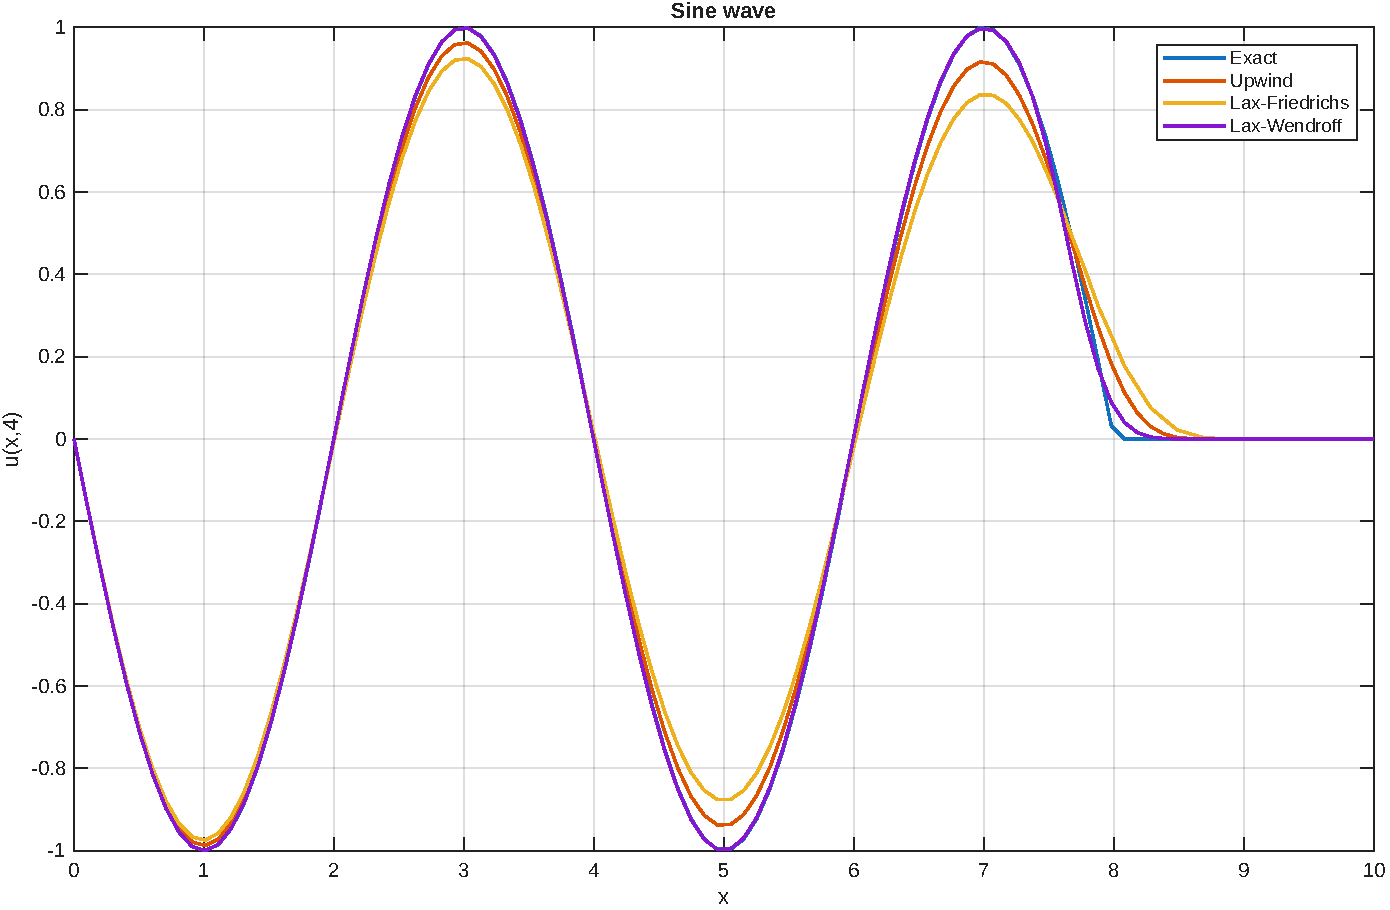
\includegraphics[width=0.92\linewidth]{part1_sine_comparison.pdf}
\caption{Exact and numerical solutions for the sine inflow at $t=4$.}
\label{fig:sine-comparison}
\end{figure}

For the smooth sine wave, Lax--Wendroff follows the exact amplitude and phase
most closely. Upwind damps the amplitude moderately, while Lax--Friedrichs is
the most strongly smeared. At the wave front $x=8$, all numerical schemes
replace the abrupt transition to the zero initial state by a finite-width
transition layer.

\begin{figure}[htbp]
\centering
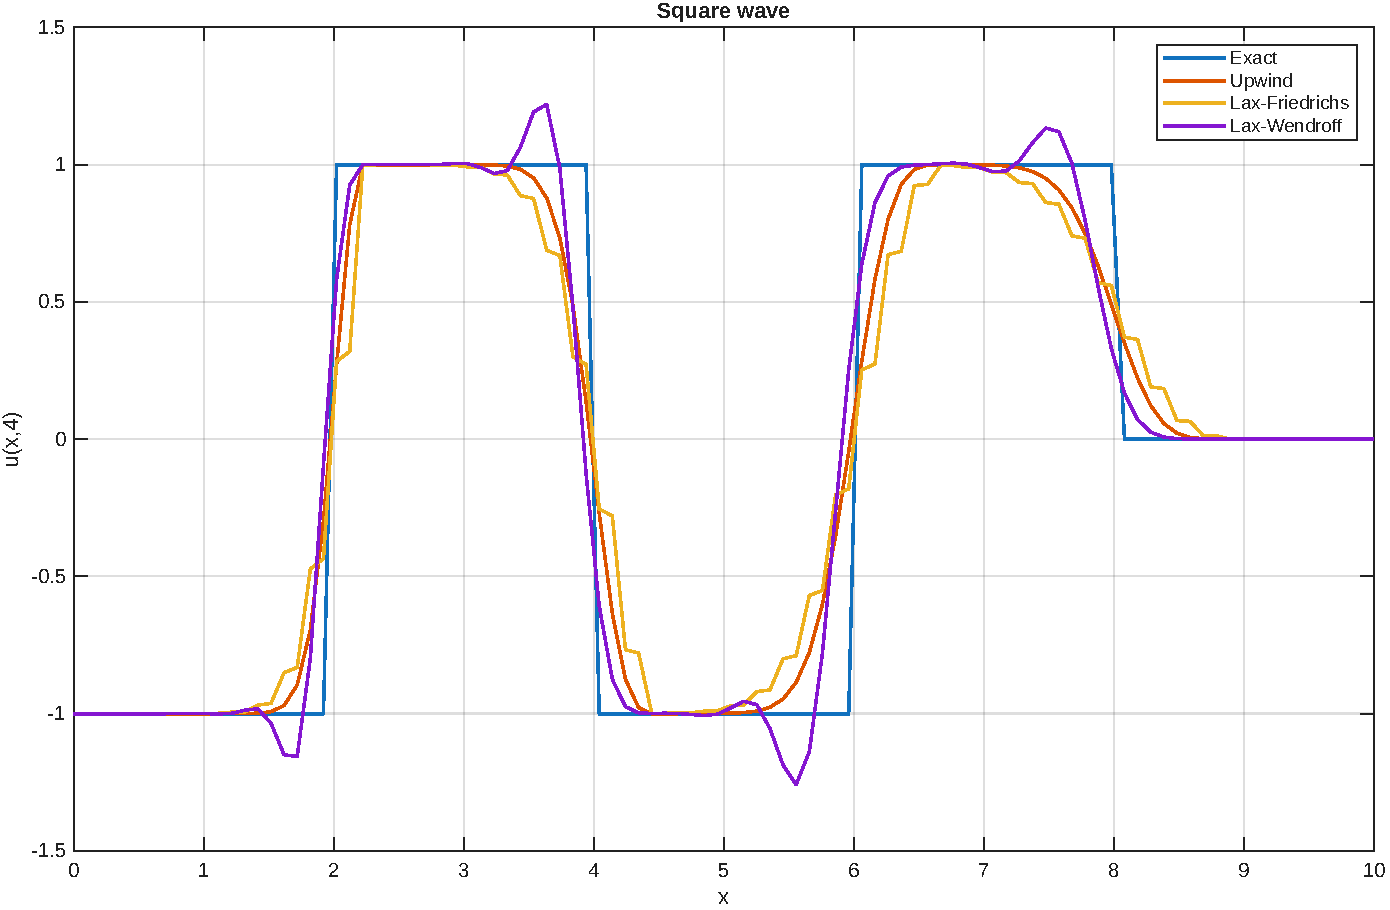
\includegraphics[width=0.92\linewidth]{part1_square_comparison.pdf}
\caption{Exact and numerical solutions for the square-wave inflow at $t=4$.}
\label{fig:square-comparison}
\end{figure}

For the square wave, the difference between diffusion and dispersion is clear.
Upwind rounds every jump but remains between the neighboring states.
Lax--Friedrichs spreads each jump over an even wider region. Lax--Wendroff
keeps the transition relatively narrow but produces overshoots and undershoots
of roughly 30 percent near the discontinuities.

\begin{table}[htbp]
\centering
\caption{Errors at $t=4$ for $N_x=100$ and $\lambda=0.9$. The discrete
$L^2$ norm is $(h\sum_j|e_j|^2)^{1/2}$.}
\begin{tabular}{@{}llccc@{}}
\toprule
Boundary data & Error norm & Upwind & Lax--Friedrichs & Lax--Wendroff\\
\midrule
Sine & $L^2$ & 0.1277 & 0.2392 & 0.0383\\
Sine & $L^\infty$ & 0.1513 & 0.2195 & 0.0574\\
Square & $L^2$ & 0.7740 & 0.9032 & 0.7841\\
Square & $L^\infty$ & 0.9552 & 0.8188 & 1.2513\\
\bottomrule
\end{tabular}
\label{tab:method-errors}
\end{table}

The sine-wave errors confirm the formal orders: Lax--Wendroff is clearly most
accurate on smooth data. For the square wave, a pointwise norm is dominated by
the unresolved jumps. The large Lax--Wendroff $L^\infty$ error records its
overshoot, while the first-order methods trade oscillations for smearing.

\FloatBarrier
\section{Part 1(d): CFL and grid experiments}

\subsection{Fixed spatial grid and different CFL numbers}

The first experiment fixes $N_x=100$ and applies upwind to the sine inflow with
\[
 \lambda\in\{0.2,0.4,0.8,0.9\}.
\]
All four values satisfy the stability condition and, for the chosen parameters,
all runs end exactly at $t=4$.

\begin{figure}[htbp]
\centering
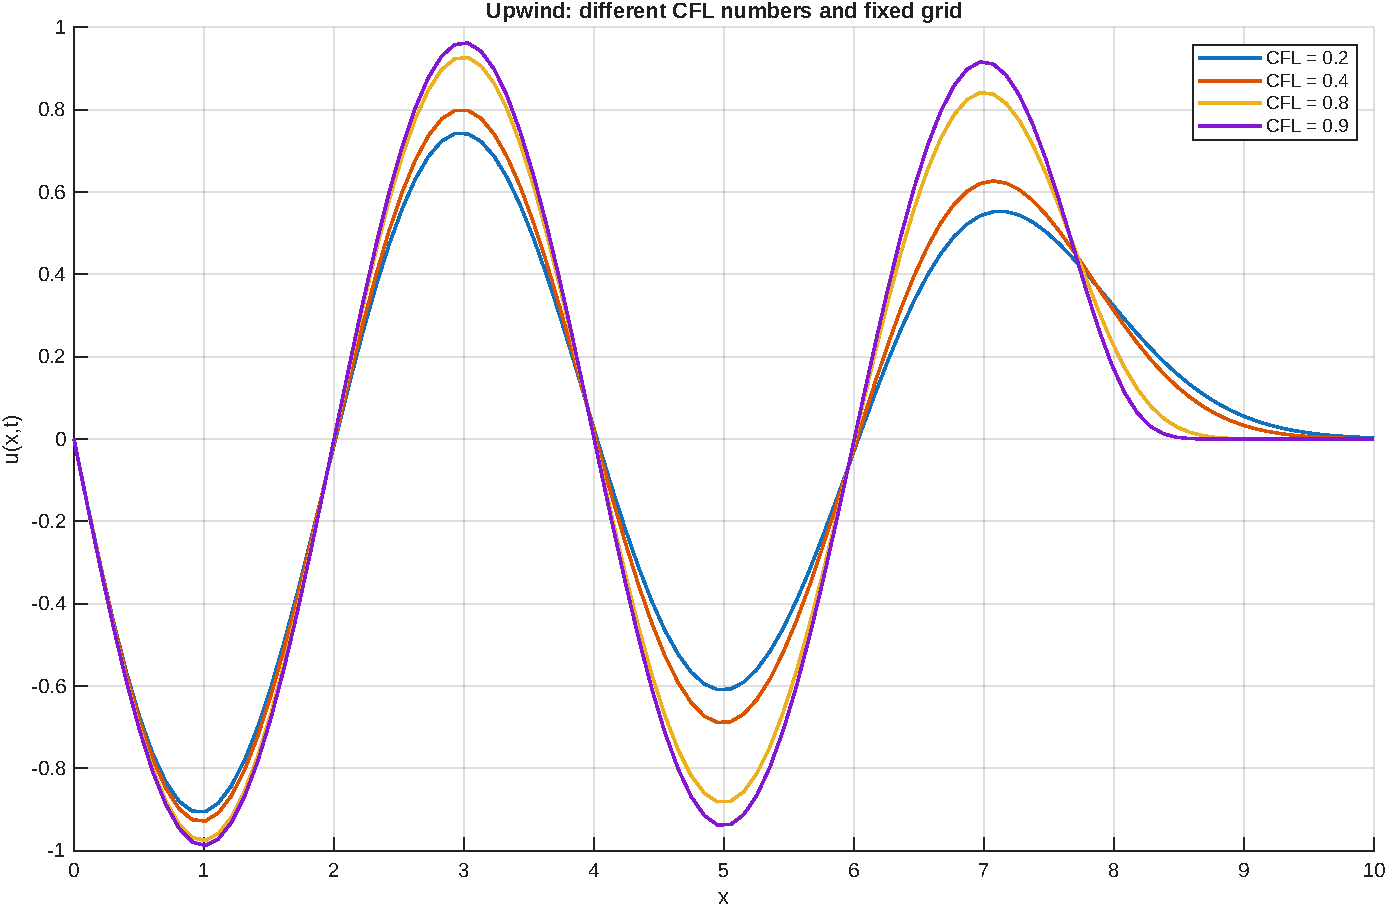
\includegraphics[width=0.92\linewidth]{part1_cfl_comparison.pdf}
\caption{Upwind solutions on the same spatial grid for different CFL numbers.}
\label{fig:cfl-comparison}
\end{figure}

Equation~\eqref{eq:upwind-modified} predicts the ordering in
Figure~\ref{fig:cfl-comparison}. The numerical viscosity is proportional to
$1-\lambda$. The run with $\lambda=0.2$ is therefore the most strongly damped,
whereas $\lambda=0.9$ stays closest to the exact amplitude. If
$\lambda>1$ is tested, the convex-combination property is lost and Fourier
modes grow, in agreement with the CFL stability restriction.

The special choice $\lambda=1$ gives
\[
 u_j^{n+1}=u_{j-1}^n.
\]
The numerical solution is then shifted by exactly one grid cell per time step,
which reproduces this constant-speed model problem exactly at the grid points.

\subsection{Fixed CFL number and different grids}

The second experiment fixes $\lambda=0.8$ and uses
\[
 N_x\in\{50,100,200,400\}.
\]
Since $k=\lambda h/a$, refining the spatial grid also refines the time step in
the same proportion. With the present parameters, each run again ends exactly
at $t=4$.

\begin{figure}[H]
\centering
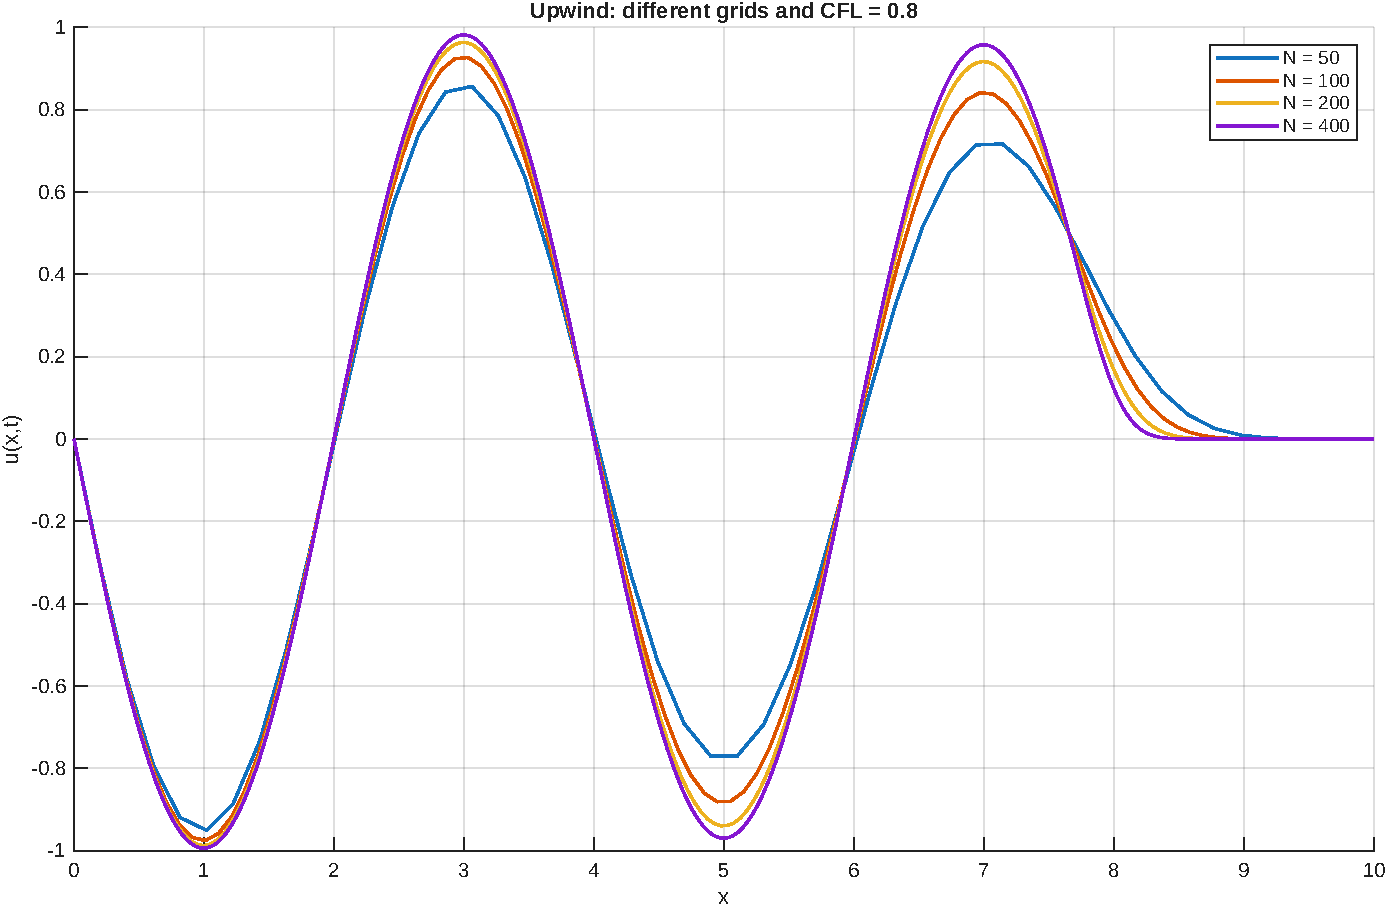
\includegraphics[width=0.68\linewidth]{part1_grid_comparison.pdf}
\caption{Upwind solutions with fixed CFL number $0.8$ on successively finer grids.}
\label{fig:grid-comparison}
\end{figure}

At fixed $\lambda$, equation~\eqref{eq:upwind-modified} shows that the
artificial viscosity is proportional to $h$. The coarse-grid solution is
therefore visibly damped, while the $N_x=400$ curve is much closer to the exact
sine wave and has a sharper wave front at $x=8$.

\begin{table}[H]
\centering
\caption{Grid refinement for upwind with sine inflow and $\lambda=0.8$.}
\begin{tabular}{@{}ccc@{}}
\toprule
$N_x$ & Discrete $L^2$ error & Observed rate\\
\midrule
50  & 0.40556 & --\\
100 & 0.23046 & 0.815\\
200 & 0.12781 & 0.850\\
400 & 0.07027 & 0.863\\
\bottomrule
\end{tabular}
\label{tab:grid-errors}
\end{table}

The rates move toward the formal first-order rate. They are somewhat below one
because the solution is only piecewise smooth at the leading wave front, where
the incoming sine wave meets the zero initial state.

\FloatBarrier
\section{Part 1 conclusions}

The model problem transports boundary data along the straight characteristics
$x-at=C$. Since $a>0$, information enters at $x=0$, travels with speed $a$, and
has reached only $x=8$ by $t=4$.

All three finite-difference methods are stable under the CFL restriction
$\lambda\leq1$. Their error mechanisms are nevertheless different:
\begin{itemize}
 \item Upwind is stable and nonoscillatory but introduces numerical diffusion.
 \item Lax--Friedrichs introduces still more diffusion and gives the most
 smeared solutions in these experiments.
 \item Lax--Wendroff is second-order accurate and best for the smooth sine wave,
 but its dispersive error creates oscillations near square-wave jumps.
\end{itemize}

\clearpage
\section{Part 2(a): water-wave system and its characteristics}

\subsection{Standard vector form}

The linearized Saint--Venant equations are
\begin{align}
 u_t+u_x+\alpha v_x&=0,\\
 v_t+\alpha u_x+v_x&=f.
\end{align}
The letter $v$ already denotes the scalar velocity perturbation, so we use
$\mathbf q$ for the vector of unknowns. The standard form is
\begin{equation}
 \boxed{\mathbf q_t+A\mathbf q_x=\mathbf F},
\end{equation}
where
\begin{equation}
 \boxed{
 \mathbf q=\begin{bmatrix}u\\v\end{bmatrix},
 \qquad
 A=\begin{bmatrix}1&\alpha\\ \alpha&1\end{bmatrix},
 \qquad
 \mathbf F=\begin{bmatrix}0\\f\end{bmatrix}.}
 \label{eq:part2-standard-form}
\end{equation}
Indeed,
\[
 A\mathbf q_x
 =\begin{bmatrix}1&\alpha\\ \alpha&1\end{bmatrix}
  \begin{bmatrix}u_x\\v_x\end{bmatrix}
 =\begin{bmatrix}u_x+\alpha v_x\\ \alpha u_x+v_x\end{bmatrix},
\]
which reproduces the spatial terms in the two equations.

\subsection{Why the eigenvalues are characteristic speeds}

For the scalar equation $z_t+c z_x=0$, information is constant along the
straight characteristics $x-ct=C$. Therefore, if the system can be rewritten
as independent scalar advection equations, the advection coefficients in
those equations are its characteristic speeds.

The eigenvalues of $A$ satisfy
\begin{align}
 0&=\det(A-\lambda I)\\
  &=\det\begin{bmatrix}1-\lambda&\alpha\\
                \alpha&1-\lambda\end{bmatrix}\\
  &=(1-\lambda)^2-\alpha^2.
\end{align}
Thus
\begin{equation}
 \boxed{\lambda_+=1+\alpha,
 \qquad \lambda_-=1-\alpha.}
 \label{eq:part2-eigenvalues}
\end{equation}
Associated eigenvectors are
\[
 r_+=\begin{bmatrix}1\\1\end{bmatrix},
 \qquad
 r_-=\begin{bmatrix}1\\-1\end{bmatrix}.
\]

The same result can be seen without matrix notation. Define the characteristic
variables
\begin{equation}
 w_+=u+v,
 \qquad
 w_-=u-v.
\end{equation}
Adding the original equations gives
\begin{equation}
 (w_+)_t+(1+\alpha)(w_+)_x=f,
 \label{eq:wplus}
\end{equation}
whereas subtracting the second equation from the first gives
\begin{equation}
 (w_-)_t+(1-\alpha)(w_-)_x=-f.
 \label{eq:wminus}
\end{equation}
The coupled system has therefore become two scalar advection equations. Their
transport speeds are exactly the eigenvalues in
equation~\eqref{eq:part2-eigenvalues}. The source $f$ creates disturbances in
the two modes, but it does not change their propagation speeds.

For $\mathrm{Fr}=0.35$,
\[
 \alpha=\frac{1}{\mathrm{Fr}}
 =\frac{1}{0.35}=\frac{20}{7}.
\]
Consequently,
\begin{equation}
 \boxed{
 \lambda_+=\frac{27}{7}\approx3.8571,
 \qquad
 \lambda_-=-\frac{13}{7}\approx-1.8571.}
 \label{eq:part2-speeds}
\end{equation}
Both eigenvalues are real and distinct, so the system is strictly hyperbolic.
Their signs show the geometry directly: the $w_+$ mode travels to the right,
while the $w_-$ mode travels to the left.

\begin{table}[htbp]
\centering
\caption{Characteristic modes of the water-wave system.}
\begin{tabular}{@{}lccc@{}}
\toprule
Mode & Characteristic variable & Speed & Direction\\
\midrule
$+$ & $w_+=u+v$ & $27/7$ & Right\\
$-$ & $w_-=u-v$ & $-13/7$ & Left\\
\bottomrule
\end{tabular}
\end{table}

\subsection{CFL condition from characteristic motion}

Let the spatial and temporal step sizes be $\Delta x$ and $\Delta t$. During
one time step, a characteristic with speed $\lambda_i$ travels the physical
distance
\begin{equation}
 |\lambda_i|\Delta t.
\end{equation}
The explicit nearest-neighbor schemes use information from at most one grid
cell away during one step. Their numerical domain of dependence can contain
the physical domain of dependence only if
\begin{equation}
 |\lambda_i|\Delta t\leq\Delta x
 \qquad\text{for every characteristic family.}
 \label{eq:part2-cfl-each}
\end{equation}
This is the same CFL argument as for scalar advection, but it must now hold for
both scalar equations~\eqref{eq:wplus}--\eqref{eq:wminus}. Therefore the
fastest absolute characteristic speed controls the step size:
\begin{equation}
 \frac{\Delta t}{\Delta x}
 \max_i|\lambda_i|\leq1.
\end{equation}
Using equation~\eqref{eq:part2-speeds},
\[
 \max_i|\lambda_i|
 =\max\left\{\frac{27}{7},\frac{13}{7}\right\}
 =\frac{27}{7}.
\]
Hence
\begin{equation}
 \frac{27}{7}\frac{\Delta t}{\Delta x}\leq1,
\end{equation}
or equivalently
\begin{equation}
 \boxed{
 \Delta t\leq c\Delta x,
 \qquad
 c=\frac{7}{27}\approx0.25926.}
 \label{eq:part2-cfl-final}
\end{equation}
The prescribed source does not add a propagation-speed restriction because it
acts locally and is not a stiff evolution term in the unknowns.

\subsection{Time until a wave reaches an artificial boundary}

This calculation uses the same characteristic geometry as Part 1. A wave mode
with speed $\lambda$ generated at position $x_0$ and time zero follows
\begin{equation}
 x(t)=x_0+\lambda t.
 \label{eq:part2-characteristic-path}
\end{equation}
The spatial source is supported in
\[
 |x|<\frac{1}{20},
\]
so waves can be generated throughout $-0.05<x<0.05$. To obtain the earliest
possible boundary contact, we start each wave at the edge of the source region
closest to the boundary toward which it travels.

For the right boundary $L_1=0.7$, the right-moving mode begins as far right as
$x_0=0.05$. Its arrival time satisfies
\begin{align}
 0.7&=0.05+\frac{27}{7}T_{\mathrm{right}},\\
 T_{\mathrm{right}}
 &=\frac{0.7-0.05}{27/7}
 =0.65\frac{7}{27}
 =\frac{91}{540}
 \approx0.16852.
\end{align}

For the left boundary $L_0=-0.4$, the left-moving mode begins as far left as
$x_0=-0.05$. Its arrival time satisfies
\begin{align}
 -0.4&=-0.05-\frac{13}{7}T_{\mathrm{left}},\\
 T_{\mathrm{left}}
 &=\frac{0.35}{13/7}
 =0.35\frac{7}{13}
 =\frac{49}{260}
 \approx0.18846.
\end{align}
The earliest influence of an artificial boundary is therefore
\begin{equation}
 \boxed{
 T^*=\min\{T_{\mathrm{right}},T_{\mathrm{left}}\}
 =T_{\mathrm{right}}
 \approx0.16852>0.15.}
 \label{eq:part2-boundary-time}
\end{equation}

As a direct geometric check, at $t=0.15$ the two outermost wave fronts are
\begin{align}
 x_{\mathrm{right}}(0.15)
 &=0.05+\frac{27}{7}(0.15)
 \approx0.6286<0.7,\\
 x_{\mathrm{left}}(0.15)
 &=-0.05-\frac{13}{7}(0.15)
 \approx-0.3286>-0.4.
\end{align}
Both fronts are still strictly inside the computational interval. Therefore
the artificial boundary conditions cannot affect the solution during the
required simulation interval $0\leq t\leq0.15$.

\clearpage
\section{Part 2(b): analytical integral solution}

\subsection{Forced advection along a characteristic}

The integral formulas follow from the same characteristic calculation as in
Part 1. Consider first the scalar forced advection equation
\begin{equation}
 z_t+c z_x=r(x,t),
 \qquad z(x,0)=0.
 \label{eq:forced-advection}
\end{equation}
The backward characteristic through $(x,t)$ is
\begin{equation}
 X(s)=x-c(t-s),
 \qquad X(t)=x,
 \qquad X'(s)=c.
\end{equation}
Along this curve, the total derivative is
\begin{align}
 \frac{\dd}{\dd s}z(X(s),s)
 &=z_x(X(s),s)X'(s)+z_t(X(s),s)\\
 &=z_t+c z_x\\
 &=r(X(s),s).
\end{align}
Integration from $s=0$ to $s=t$ gives
\begin{align}
 z(x,t)-z(x-ct,0)
 &=\int_0^t r\bigl(x-c(t-s),s\bigr)\,\dd s.
\end{align}
The initial value vanishes, so
\begin{equation}
 \boxed{z(x,t)=\int_0^t r\bigl(x-c(t-s),s\bigr)\,\dd s.}
 \label{eq:duhamel-characteristic}
\end{equation}
The argument $x-c(t-s)$ is the position at the earlier time $s$ of the
characteristic that arrives at $x$ at time $t$.

\subsection{Application to the two characteristic variables}

Equations~\eqref{eq:wplus}--\eqref{eq:wminus} have zero initial data and are
of the form~\eqref{eq:forced-advection}. Define
\begin{align}
 I_+(x,t)
 &=\int_0^t f\bigl(x-(1+\alpha)(t-s),s\bigr)\,\dd s,\\
 I_-(x,t)
 &=\int_0^t f\bigl(x-(1-\alpha)(t-s),s\bigr)\,\dd s.
\end{align}
Then
\begin{equation}
 w_+=I_+,
 \qquad
 w_-=-I_-,
\end{equation}
because the source in the $w_-$ equation is $-f$. Since
\[
 u=\frac{w_++w_-}{2},
 \qquad
 v=\frac{w_+-w_-}{2},
\]
we recover the stated analytical solution:
\begin{equation}
 \boxed{
 u(x,t)=\frac12\left(I_+(x,t)-I_-(x,t)\right),
 \qquad
 v(x,t)=\frac12\left(I_+(x,t)+I_-(x,t)\right).}
 \label{eq:part2-analytical}
\end{equation}

The remaining one-dimensional integrals are evaluated with \matlab's
\texttt{integral} routine using relative tolerance $10^{-10}$ and absolute
tolerance $10^{-12}$. These tolerances are much smaller than the finite-
difference errors reported below, so quadrature error does not determine the
comparison.

\section{Part 2(c): numerical solution of the system}

\subsection{Grid and matrix splitting}

The computation uses $N_x=400$ points on $[-0.4,0.7]$, hence
\begin{equation}
 \Delta x=\frac{1.1}{399}\approx2.75689\cdot10^{-3}.
\end{equation}
Starting from a requested CFL number $0.9$, the number of steps is rounded up
so that the computation ends exactly at $T=0.15$. This gives
\begin{equation}
 N_t=234,
 \qquad
 \Delta t=\frac{0.15}{234}\approx6.41026\cdot10^{-4},
 \qquad
 \frac{27}{7}\frac{\Delta t}{\Delta x}\approx0.89685<1.
\end{equation}

For system upwind, diagonalization separates the two propagation directions:
\begin{equation}
 A=S\Lambda S^{-1},
 \qquad
 A^+=S\Lambda^+S^{-1},
 \qquad
 A^-=S\Lambda^-S^{-1}.
\end{equation}
Here $\Lambda^+$ keeps only positive eigenvalues and $\Lambda^-$ keeps only
negative eigenvalues. With the present values,
\begin{equation}
 A^+=\frac{27}{14}
 \begin{bmatrix}1&1\\1&1\end{bmatrix},
 \qquad
 A^-=\frac{-13}{14}
 \begin{bmatrix}1&-1\\-1&1\end{bmatrix}.
 \label{eq:part2-matrix-parts}
\end{equation}
Thus $A^+$ applies the backward difference to the right-moving mode, whereas
$A^-$ applies the forward difference to the left-moving mode.

\subsection{System upwind and Lax--Wendroff schemes}

Write $\mu=\Delta t/\Delta x$. The system upwind method is
\begin{equation}
 \boxed{
 \mathbf q_j^{n+1}=\mathbf q_j^n
 -\mu A^+(\mathbf q_j^n-\mathbf q_{j-1}^n)
 -\mu A^-(\mathbf q_{j+1}^n-\mathbf q_j^n)
 +\Delta t\,\mathbf F_j^n.}
 \label{eq:part2-upwind}
\end{equation}
Each characteristic family is therefore differenced from the direction from
which its information arrives.

The Lax--Wendroff method is
\begin{align}
 \mathbf q_j^{n+1}
 ={}&\mathbf q_j^n
 -\frac{\mu}{2}A(\mathbf q_{j+1}^n-\mathbf q_{j-1}^n)\nonumber\\
 &+\frac{\mu^2}{2}A^2
 (\mathbf q_{j+1}^n-2\mathbf q_j^n+\mathbf q_{j-1}^n)
 +\Delta t\,\widetilde{\mathbf F}_j^n,
 \label{eq:part2-lw}
\end{align}
where
\begin{equation}
 \widetilde{\mathbf F}_j^n
 =\frac{\mathbf F_j^n+\mathbf F_j^{n+1}}{2}
 -\frac{\mu}{4}A(\mathbf F_{j+1}^n-\mathbf F_{j-1}^n).
 \label{eq:part2-source-correction}
\end{equation}
The time average represents the source over the entire step. The second term
accounts for spatial transport of the disturbance during that step. Omitting
this correction would destroy the intended second-order source treatment.

\subsection{Why the boundary extrapolation has this form}

The centered stencils update only the interior points. At the left endpoint,
linear extrapolation requires the two neighboring discrete slopes to agree:
\begin{equation}
 \frac{\mathbf q_1^n-\mathbf q_0^n}{\Delta x}
 =\frac{\mathbf q_2^n-\mathbf q_1^n}{\Delta x}.
\end{equation}
Solving for the boundary vector gives
\begin{equation}
 \boxed{\mathbf q_0^n=2\mathbf q_1^n-\mathbf q_2^n.}
\end{equation}
The same argument at the right endpoint gives
\begin{equation}
 \boxed{\mathbf q_N^n=2\mathbf q_{N-1}^n-\mathbf q_{N-2}^n.}
\end{equation}
This simply continues the straight line through the closest two interior
values, or equivalently imposes zero discrete curvature. It is applied to
both $u$ and $v$ after every interior time-step update. It is an artificial
numerical closure, but equation~\eqref{eq:part2-boundary-time} shows that it
cannot influence the solution before $t=0.15$.

\subsection{Final-time comparison}

\begin{figure}[htbp]
\centering
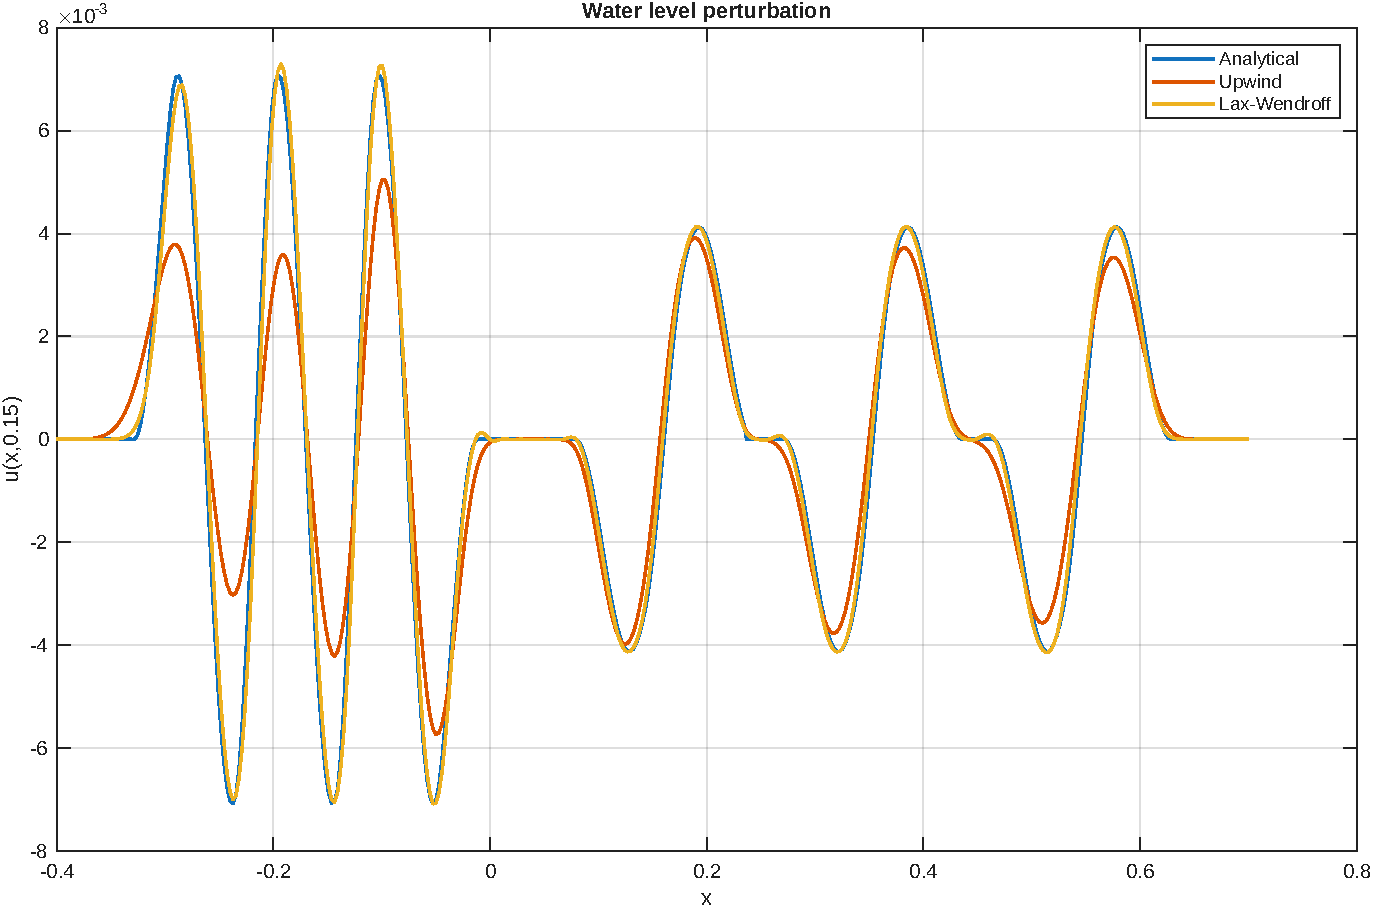
\includegraphics[width=0.94\linewidth]{part2_u_comparison.pdf}
\caption{Analytical, upwind, and Lax--Wendroff approximations of the water-level
perturbation at $t=0.15$.}
\label{fig:part2-u}
\end{figure}

\begin{figure}[htbp]
\centering
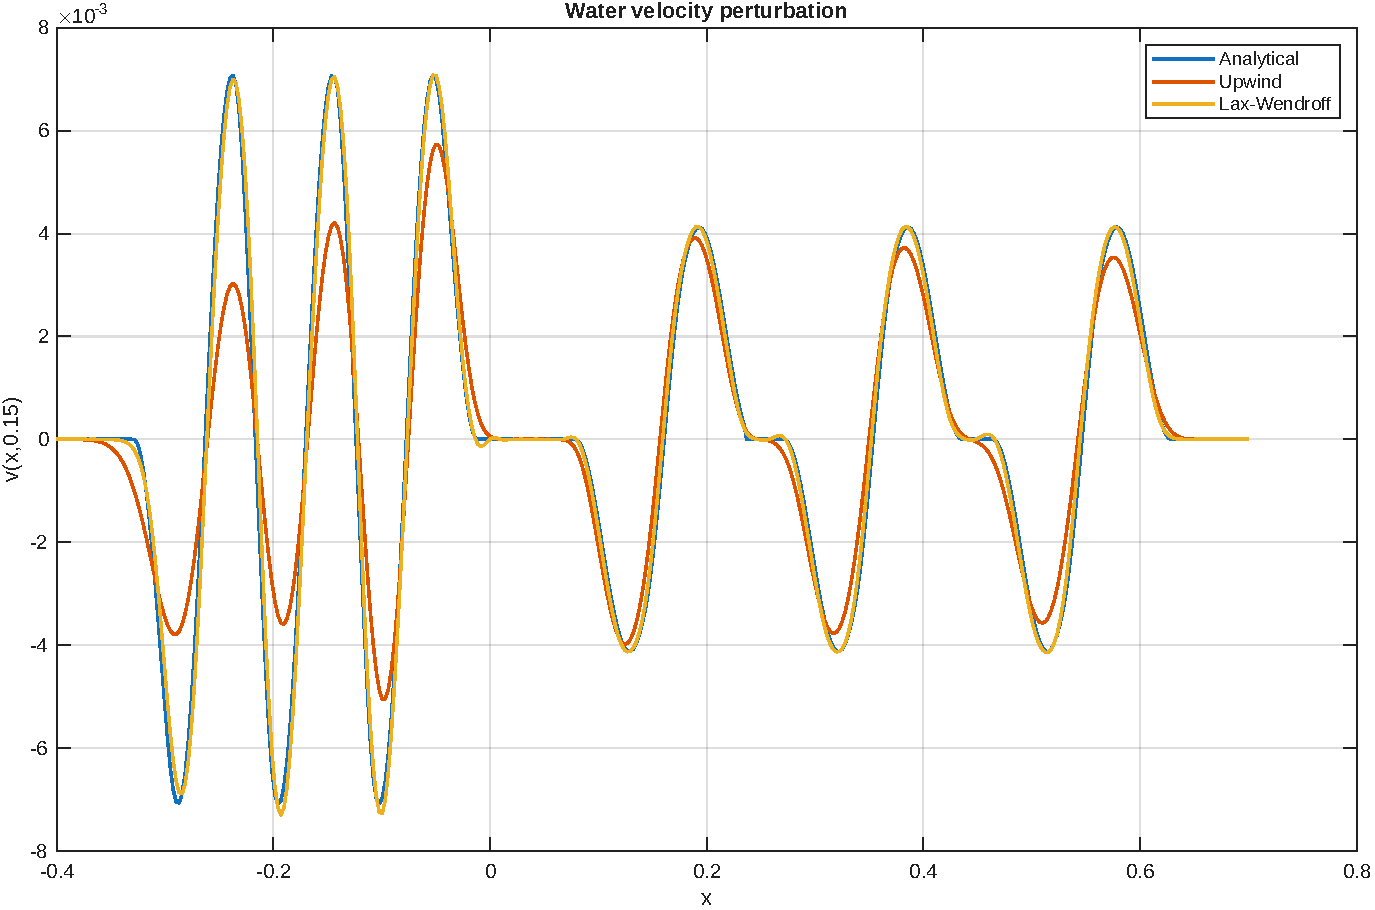
\includegraphics[width=0.94\linewidth]{part2_v_comparison.pdf}
\caption{Analytical, upwind, and Lax--Wendroff approximations of the velocity
perturbation at $t=0.15$.}
\label{fig:part2-v}
\end{figure}

The upwind method remains nonoscillatory but visibly reduces the amplitude and
widens the pulses, particularly in the left-moving train. Lax--Wendroff follows
the analytical peaks and phase much more closely. Its small ripples near the
ends of the wave packets are the same dispersive behavior seen near
discontinuities in Part 1.

\begin{table}[htbp]
\centering
\caption{Maximum errors at $t=0.15$ for $N_x=400$.}
\begin{tabular}{@{}lcc@{}}
\toprule
Variable & Upwind & Lax--Wendroff\\
\midrule
$u$ & $4.0528\cdot10^{-3}$ & $1.0607\cdot10^{-3}$\\
$v$ & $4.0528\cdot10^{-3}$ & $1.0607\cdot10^{-3}$\\
\bottomrule
\end{tabular}
\label{tab:part2-final-errors}
\end{table}

\FloatBarrier
\subsection{Propagation speeds and wave structure}

\begin{figure}[htbp]
\centering
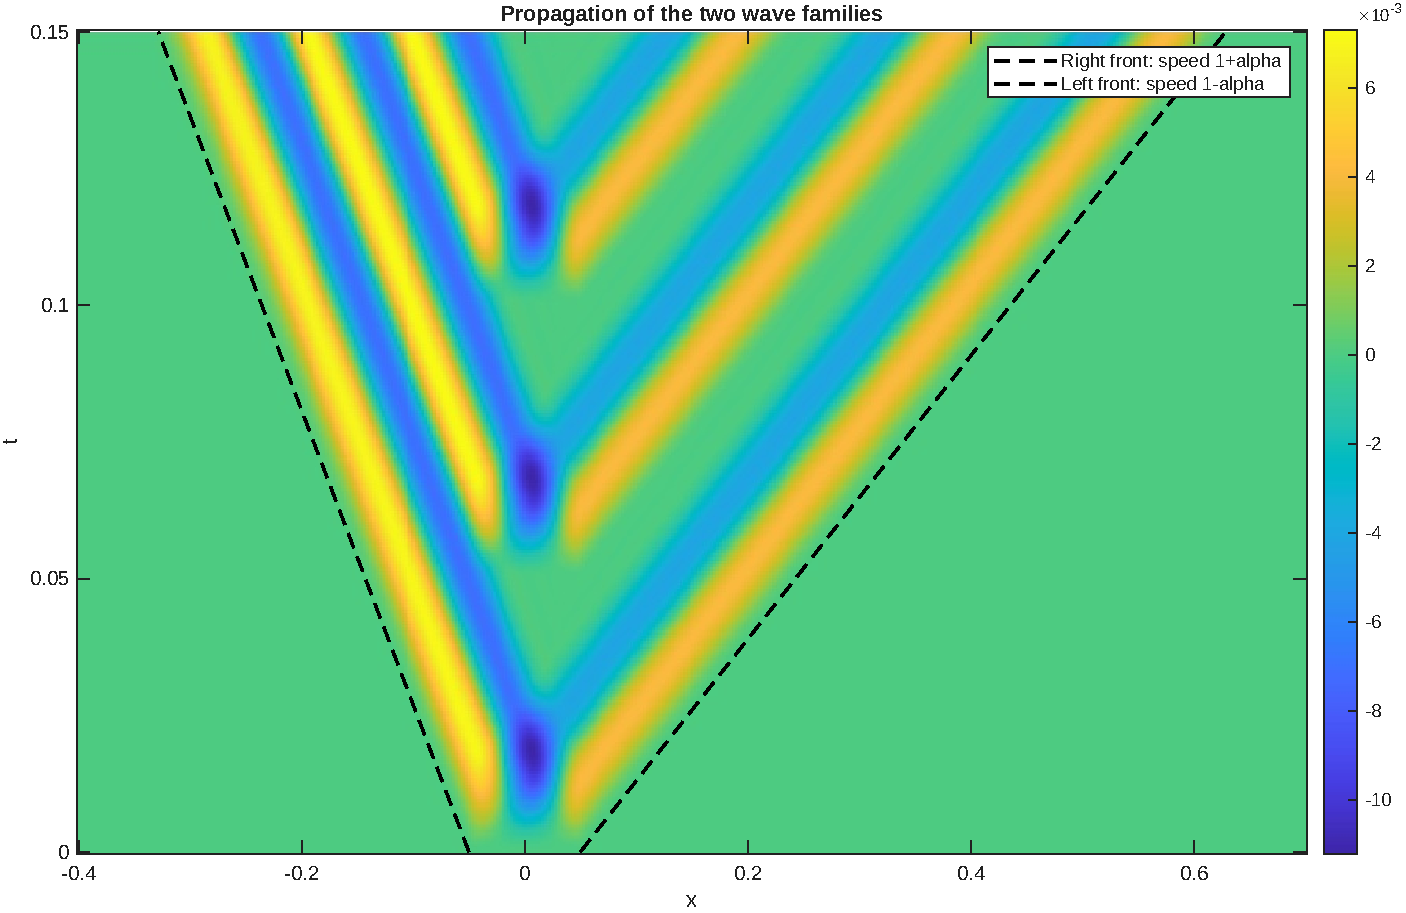
\includegraphics[width=0.94\linewidth]{part2_propagation.pdf}
\caption{Space--time view of the Lax--Wendroff solution for $u$. The dashed
curves are the two theoretical outer wave fronts.}
\label{fig:part2-propagation}
\end{figure}

In Figure~\ref{fig:part2-propagation}, the right-moving ridges have slope
$\dd x/\dd t=27/7$ and the left-moving ridges have slope $-13/7$. Their
agreement with the dashed lines is a direct visual verification of both
eigenvalue speeds.

The temporal forcing repeats with period
\begin{equation}
 T_f=\frac{2\pi}{40\pi}=\frac1{20}.
\end{equation}
Consequently the spatial repetition lengths of the two wave trains are
\begin{align}
 \ell_+&=|1+\alpha|T_f=\frac{27}{140}\approx0.19286,\\
 \ell_-&=|1-\alpha|T_f=\frac{13}{140}\approx0.09286.
\end{align}
The left-going wave therefore has the shorter spatial wavelength. Within each
wave family, repeated peaks generated by identical forcing periods have the
same analytical height. The two families do not have equal heights: at the
final time the largest magnitudes in $u$ are approximately
$7.08\cdot10^{-3}$ on the left and $4.13\cdot10^{-3}$ on the right. The slower
left-moving characteristic remains in the localized source region longer and
therefore accumulates a different integral of the forcing.

\subsection{CFL violation}

\begin{figure}[htbp]
\centering
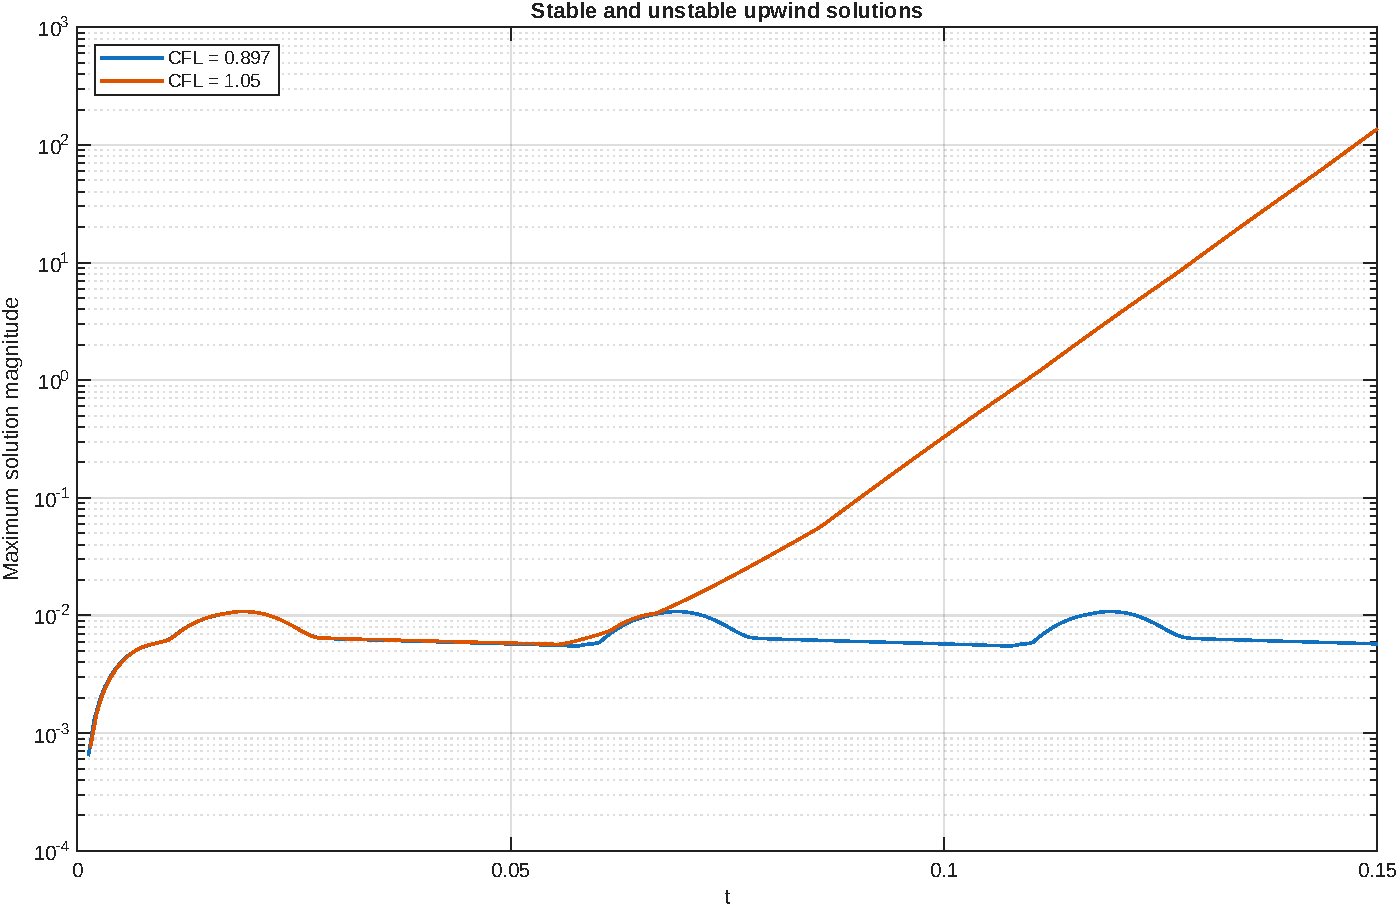
\includegraphics[width=0.88\linewidth]{part2_stability.pdf}
\caption{Maximum magnitude over both components for stable and unstable upwind
runs on the same spatial grid.}
\label{fig:part2-stability}
\end{figure}

With CFL $0.89685$, the solution remains of physical size, approximately
$10^{-2}$. With CFL $1.05$, high-frequency components grow until the maximum
solution magnitude is approximately $1.37\cdot10^2$ at $t=0.15$. The source
and its switching points continually seed grid-scale components, and the
violated amplification bound magnifies them. This experiment agrees directly
with the theoretical condition
\[
 \max_i|\lambda_i|\frac{\Delta t}{\Delta x}\leq1.
\]

\subsection{Grid refinement and choice of method}

\begin{figure}[htbp]
\centering
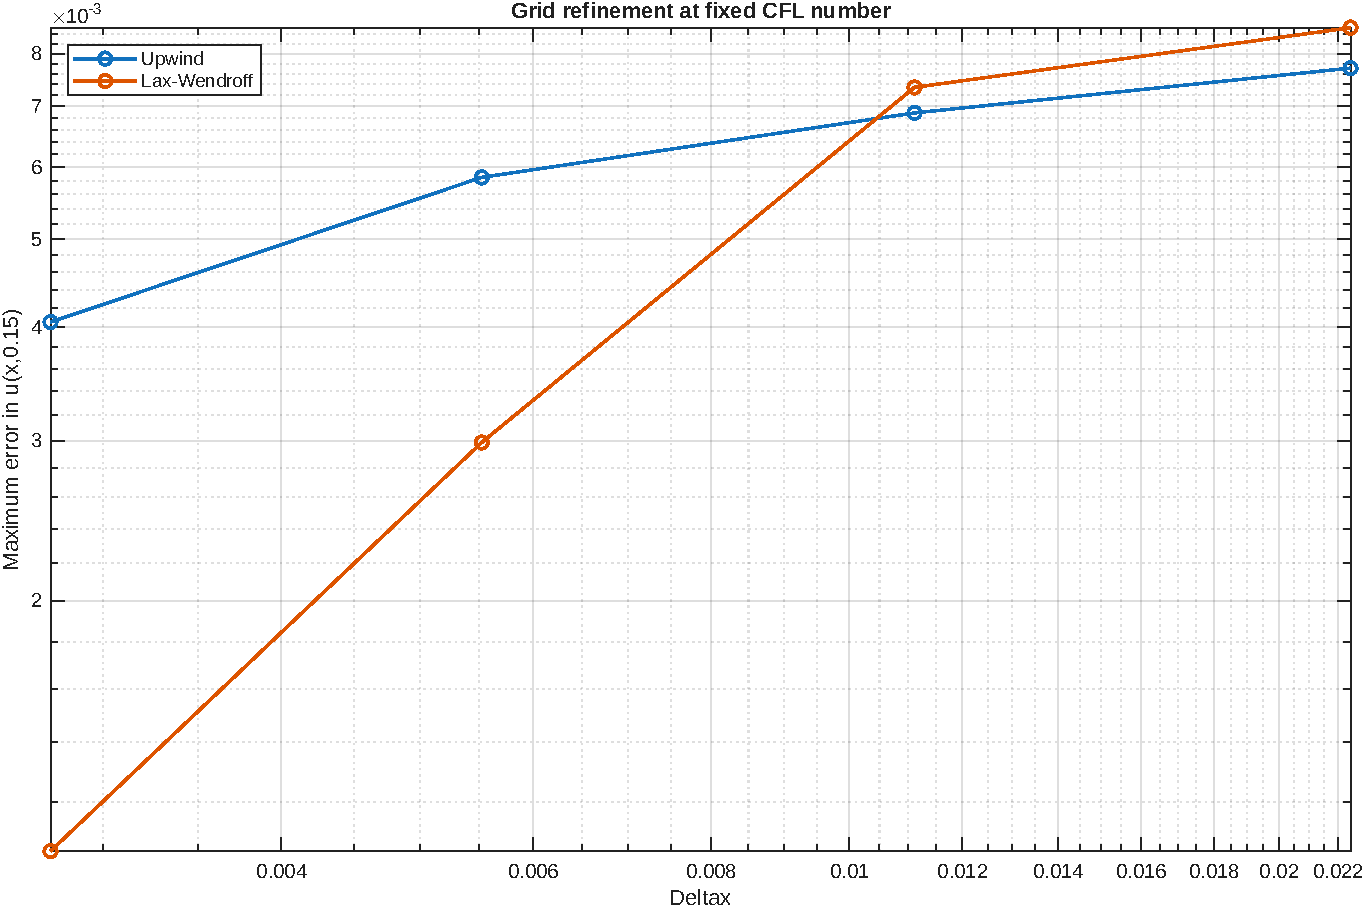
\includegraphics[width=0.88\linewidth]{part2_convergence.pdf}
\caption{Maximum error in $u(x,0.15)$ for successively refined grids at fixed
requested CFL number $0.9$.}
\label{fig:part2-convergence}
\end{figure}

\begin{table}[htbp]
\centering
\caption{Grid refinement in the maximum norm. Rates compare consecutive rows.}
\begin{tabular}{@{}rrrrr@{}}
\toprule
$N_x$ & Upwind error & Rate & Lax--Wendroff error & Rate\\
\midrule
50  & $7.7118\cdot10^{-3}$ & --    & $8.5428\cdot10^{-3}$ & --\\
100 & $6.8845\cdot10^{-3}$ & 0.161 & $7.3453\cdot10^{-3}$ & 0.215\\
200 & $5.8471\cdot10^{-3}$ & 0.234 & $2.9874\cdot10^{-3}$ & 1.289\\
400 & $4.0528\cdot10^{-3}$ & 0.527 & $1.0607\cdot10^{-3}$ & 1.489\\
\bottomrule
\end{tabular}
\label{tab:part2-refinement}
\end{table}

The coarse grids do not resolve the shorter left-going wavelength well, so
neither method is yet in a clean asymptotic regime. Once the grid is refined,
Lax--Wendroff improves much faster and is the more accurate method for this
problem. The nonsmooth on--off forcing and the maximum norm prevent the full
smooth-solution second-order rate from appearing at these resolutions.

The left-moving train is harder to approximate for two related reasons.
First, its spatial wavelength is shorter, so it has fewer grid points per
oscillation. Second, the global time step is limited by the faster right-going
speed. At global CFL $0.9$, the mode-specific CFL numbers are
\begin{equation}
 \nu_+=0.9,
 \qquad
 \nu_-=\frac{13}{27}(0.9)\approx0.433.
\end{equation}
Upwind diffusion grows as the mode CFL moves below one, so the left-going mode
is substantially more smeared. Lax--Wendroff is therefore the best method here
when accuracy is the main criterion. Upwind remains useful when a strictly
nonoscillatory answer is more important than resolving the peak heights.

\subsection{What changes for supercritical flow?}

For $\mathrm{Fr}>1$, one has $\alpha=1/\mathrm{Fr}<1$. Both characteristic
speeds are then positive:
\begin{equation}
 1+\alpha>0,
 \qquad
 1-\alpha>0.
\end{equation}
Both wave families travel downstream to the right; there is no left-going wave
train. In the upwind splitting, $A^-=0$ and both modes use backward spatial
differences. The left boundary is an inflow boundary for both characteristic
variables, while the right boundary is purely outflow. The CFL condition still
uses the fastest speed $1+\alpha$, but the boundary-arrival calculation and the
visible propagation pattern must be recomputed with both speeds directed to
the right.
